%% generato automaticamente da tools/build_tex.py --- non modificare
\chapter{Un nome per l'infinitesimo}
\label{cap:j}
\quaderno{j.dfw}{07 Jul 2009}{7}

Luglio 2009. Sette espressioni soltanto, ma è il quaderno che richiede più cautela nella lettura, perché due delle sue righe non vanno prese alla lettera. Il titolo del file — la lettera che gli ingegneri usano al posto di $\mathrm{i}$ — dice l'argomento: che cosa sia l'unità immaginaria, e se si possa raggiungerla per via di limiti.

\section{I due punti fissi dell'esponenziale complesso}

Le prime due righe sono la formula di Eulero valutata nei due punti in cui restituisce un numero reale.

\begin{espr}{1}{User}{\verificata}
\[
\cos\!\left(0\right) + \mathrm{i}\, \sin\!\left(0\right) = 1
\]
\end{espr}
La formula di Eulero in $x=0$.

\begin{espr}{2}{User}{\verificata}
\[
\cos\!\left(\pi\right) + \mathrm{i}\, \sin\!\left(\pi\right) = -1
\]
\end{espr}
E in $x=\pi$: è l'identità di Eulero nella forma $\mathrm{e}^{\mathrm{i}\pi}+1=0$.

\section{Due limiti e un nome}

Le due righe successive sono il cuore del quaderno e vanno lette con attenzione, perché così come sono scritte non sono vere nel senso ordinario.

\begin{espr}{3}{User}{}
\[
\mathrm{i} = \lim_{x \to 0} \frac{1 - \cos\!\left(x\right)}{\sin\!\left(x\right)}
\]
\end{espr}
Il rapporto vale $\tan(x/2)$ e il suo limite in zero è zero. L'identificazione con $\mathrm{i}$ è una convenzione di scrittura, non un'uguaglianza numerica.

\begin{espr}{4}{User}{}
\[
-\mathrm{i} = \lim_{x \to \pi} \frac{1 + \cos\!\left(x\right)}{\sin\!\left(x\right)}
\]
\end{espr}
Il rapporto vale $\cot(x/2)$ e il suo limite in $\pi$ è zero, per la stessa ragione e con segno convenzionalmente opposto.

\begin{figure}[htbp]
  \centering
  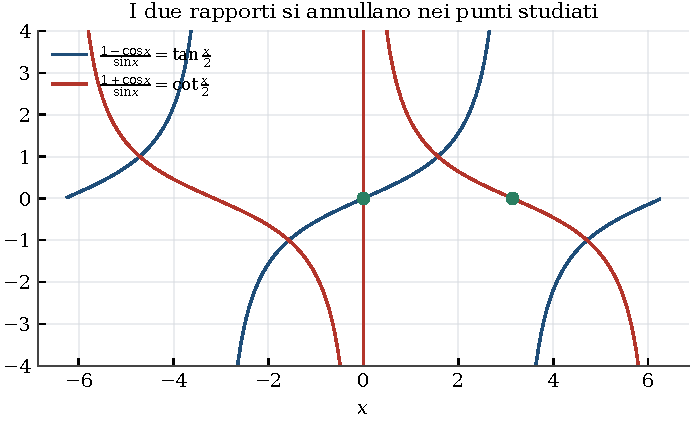
\includegraphics[width=0.86\linewidth]{../figures/j_tan.pdf}
  \caption{I due rapporti delle righe $\#3$ e $\#4$ coincidono con $\tan(x/2)$ e $\cot(x/2)$. I cerchi segnano i punti in cui vengono valutati i limiti: in entrambi il valore è zero.}
  \label{fig:j_tan}
\end{figure}

Entrambe le espressioni a secondo membro si semplificano con le formule di bisezione:
\[
  \frac{1-\cos x}{\sin x}=\tan\frac{x}{2},
  \qquad
  \frac{1+\cos x}{\sin x}=\cot\frac{x}{2}.
\]
Il primo tende a $\tan 0=0$ per $x\to0$; il secondo tende a $\cot(\pi/2)=0$ per $x\to\pi$. Nel senso ordinario dell'analisi entrambi i limiti valgono zero, e Derive stesso risponde zero se glielo si chiede.

Che cosa intendeva allora l'autore scrivendo $\mathrm{i}$ e $-\mathrm{i}$? La lettura più coerente con il resto della raccolta è che si tratti di un battesimo, non di un'uguaglianza: alle due quantità infinitesime prodotte dai due limiti viene dato un nome, esattamente come nel quaderno del maggio precedente si dava il nome $\varepsilon$ al difetto di un'operazione (capitolo~\ref{cap:teoria}). Il segno opposto distingue i due lati.

C'è però anche una lettura più tecnica, e vale la pena di indicarla. La quantità $\tan(x/2)$ è il parametro della sostituzione di Weierstrass, quella che parametrizza razionalmente il cerchio unitario e che ricomparirà in \dfw{gauss.dfw} e in \dfw{delta.dfw} nella forma $\mathrm{e}^{\mathrm{i}x}=\big(1+\mathrm{i}\tan\tfrac{x}{2}\big)^2\big/\big(1+\tan^2\tfrac{x}{2}\big)$. In quella parametrizzazione $x=0$ e $x=\pi$ sono precisamente i due punti in cui l'esponenziale vale $+1$ e $-1$: le righe $\#3$ e $\#4$ marcano quei due punti, che sono gli stessi delle righe $\#1$ e $\#2$.

\section{Che cosa succede elevando a potenza}

Le ultime tre righe mettono alla prova l'oggetto appena battezzato: che cosa gli accade se lo si eleva a una potenza che cresce?

\begin{espr}{5}{User}{\verificata}
\[
\cos\!\left(x\right) + \mathrm{i}\, \sin\!\left(x\right) = \mathrm{e}^{\mathrm{i}\, x}
\]
\end{espr}
La formula di Eulero in forma generale: la riga che dà senso alle due precedenti.

\begin{espr}{6}{User}{}
\[
\lim_{n \to +\infty} \left(\lim_{x \to 0} \frac{1 - \cos\!\left(x\right)}{\sin\!\left(x\right)}\right)^{n}
\]
\end{espr}
L'oggetto battezzato, elevato a una potenza che tende all'infinito.

\begin{espr}{7}{User}{}
\[
\left(\frac{1 - \cos\!\left(10^{-x}\right)}{\sin\!\left(10^{-x}\right)}\right)^{x}
\]
\end{espr}
La versione calcolabile: argomento $10^{-x}$ ed esponente $x$. La quantità decresce come $10^{-x^2}$.


La riga $\#7$ è la versione concreta e calcolabile della domanda: si prende l'argomento $x=10^{-n}$, cioè lo si fa tendere a zero per potenze di dieci, e si eleva alla $n$. Poiché $\tan(10^{-n}/2)\approx 10^{-n}/2$, la quantità vale circa $10^{-n^2}2^{-n}$: non tende a zero come una potenza, ma come una gaussiana negli esponenti. Se l'oggetto fosse davvero $\mathrm{i}$, il suo modulo resterebbe $1$ per sempre; il fatto che collassi così rapidamente è la prova che infinitesimo e unità immaginaria non sono la stessa cosa. Il quaderno, che è del 2009, non torna sull'argomento.

\section*{In sintesi}
\addcontentsline{toc}{section}{In sintesi}

Sette righe che pongono una domanda legittima — l'unità immaginaria si può ottenere come limite di quantità reali? — e le danno una risposta implicita ma netta. No, e la riga $\#7$ mostra perché: ciò che quei limiti producono ha modulo che tende a zero, mentre $\mathrm{i}$ ha modulo uno. La risposta affermativa arriverà, ma da un'altra strada: nel quaderno \dfw{e.dfw} dell'agosto 2010 (capitolo~\ref{cap:e}, righe $\#88$--$\#92$), dove $\mathrm{i}$ si ottiene come limite di $\left(1+\tfrac{\mathrm{i}\pi}{2x}\right)^x$ — cioè lasciando l'unità immaginaria nella formula fin dall'inizio.

